% first example chapter
% @author Thomas Lehmann
%
\chapter{Entwurf}
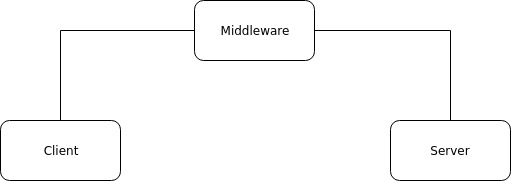
\includegraphics[scale=0.8]{../pictures/Komponenten.jpg}\\
\centerline{\textbf{Abbildung 1:} Komponentendiagramm}\\
\\Die Middleware soll dafür sorgen, dass ein entferntes Objekt wie ein lokales behandelt werden kann, ohne, dass der Anwender dies merkt. Dazu muss mit Hilfe eines Compilers und einer idl-Datei ein Stub-Objekt erzeugt werden.\\
Dieses Stub-Objekt kommuniziert über den Nameservice mit dem ObjectBroker des Servers, auf dem das richtige Objekt liegt. Die Antworten des Objektes werden direkt an ein RemoteObject, dass im Stub-Objekt die Kommunikation übernimmt, gesendet und vom Stub-Objekt in den richtigen Datentypen geparst, damit das Ergebnis direkt vom Client genutzt werden kann.\\
Der ObjectBroker vom Server, der im Nameservice hinterlegt ist, nimmt die Anfrage des Clients an und startet einen Dispatcher. Der Dispatcher leitet die Anfrage des Clients  an das passende LocalObject im MWareObjectWarehouse weiter, welches diese Anfrage parst und mittels Reflection im Objekt aufruft. Das Ergebnis dieses Aufrufs wird als String zurückgegeben und vom Dispatcher an den Client zurückgesendet.\\
\\
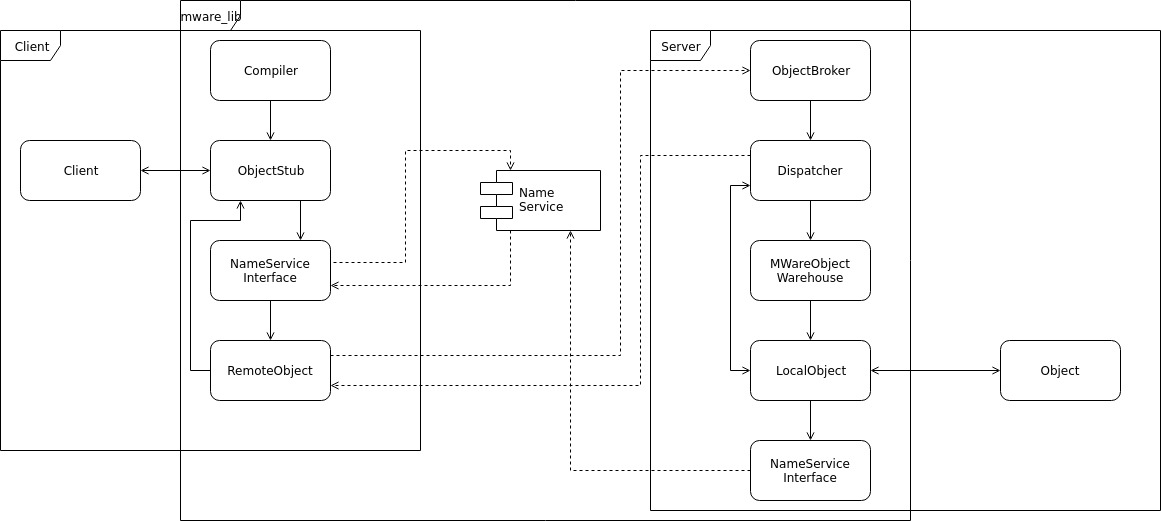
\includegraphics[scale=0.35]{../pictures/Baustein.jpg}\\
\centerline{\textbf{Abbildung 2:} Bausteindiagram Middleware}\\

\section{Protokoll}
Die Kommunikation der Middleware läuft über TCP-Sockets, daher muss ein eigenes Protokoll erstellt werden. Im folgenden wird das Protokoll beschreiben.

\subsection{Nameservice}
\subsubsection{Rebind}
Rebind bindet ein Objekt über die Hostadresse und den Port des Servers, auf dem das Objekt liegt, an den Nameservice
\begin{itemize}
\item \textbf{Aufruf:} rebind!<Name>:<Hostadresse>:<Port>
\item \textbf{Antwort:} ok
\end{itemize}

\subsubsection{Resolve}
Resolve fragt ein Objekt vom Nameservice ab. Zurückgegeben werden die Hostadresse und der Port des Servers, auf dem das angefragte Objekt liegt.
\begin{itemize}
\item \textbf{Aufruf:} resolve!<Name>
\item \textbf{Antwort:} ok:<Name>:<Hostadresse>:<Port>
\end{itemize}

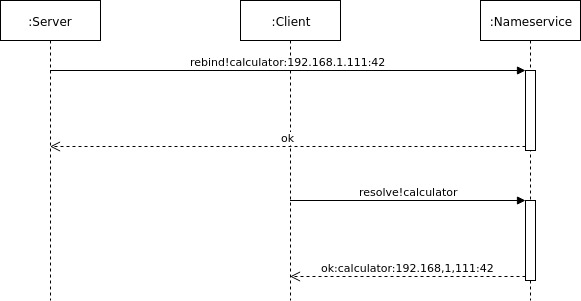
\includegraphics[scale=0.7]{../pictures/FlowChartNameService.jpg}\\
\centerline{\textbf{Abbildung 3:} Flowchart Nameservice}\\

\subsection{Middleware}
In der Middleware kommunizieren die RemoteObjekte mit den lokalen Objekten mit Hilfe des folgenden Protokolls:
\begin{itemize}
\item \textbf{Methodenaufruf:} <Objektname>!<Funktionsnname>![<Parameter>:<Datentyp>]*
\item \textbf{Antwort:} result:<Ergebnis>
\end{itemize}

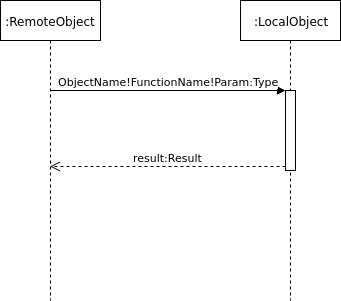
\includegraphics[scale=1]{../pictures/FlowChartObjectProtokol.jpg}\\
\centerline{\textbf{Abbildung 4:} Flowchart Objektkommunikation}\\

\subsection{Middleware}
\subsubsection{Aufruf einer Methode}
\begin{itemize}
\item \textbf{Aufruf:} resolve!<Name>
\item \textbf{Antwort:} ok:<Name>:<Hostadresse>:<Port>
\end{itemize}
 
\section{Nameservice}

Der Nameservice bildet ab, welches Objekt sich auf welchem Server befindet. Mit dem Namen des Objekts kann der Host und der Port des Servers, auf welchen das Objekt liegt, abgefragt und eine Verbindung dahin aufgebaut werden. Der Nameservice ist als entferntes Objekt zu implementieren, sodass die Nachrichtenübermittlung mittels TCP realisiert wird.

\subsection{Rebind}

\textbf{Beschreibung:}\\
Bindet ein Objekt mit dem übergebenen Namen im Nameservice.\\
Die zugehörigen Informationen sind Hostadresse und Port des Servers, auf dem das Objekt liegt. Bereits vorhandene Objekte mit dem selben Namen werden überschrieben.\\ \\
\textbf{Anfrage:} rebind!<Name>:<Hostadresse>:<Port>\\ \\
\textbf{Antwort:} ok\\ \\
\textbf{Beispiel:}
\begin{tabbing}
\textit{Server:}~~~~~~~~~~~ \= rebind!calculator:192.168.1.111:42 \\
\textit{Nameservice:} \> ok
\end{tabbing}
\textbf{Ablauf}
\begin{enumerate}
\item Auslesen von Name, Hostadresse und Port
\item Speichern der Hostadresse und des Ports unter angegebenen Namen
\item Rückgabe von ok
\end{enumerate}

\subsection{Resolve}

\textbf{Beschreibung:}\\
Fragt die zugehörigen Informationen zum Objekt mit dem übergebenen Namen ab.\\
Als Antwort werden Hostadresse und Port, die für den übergebenen Namen gespeichert wurden, zurückgegeben.\\ \\
\textbf{Anfrage:} resolve!<Name>\\ \\
\textbf{Antwort:} ok:<Name>:<Hostadresse>:<Port>\\ \\
\textbf{Beispiel:}
\begin{tabbing}
\textit{Client:}~~~~~~~~~~~ \=  resolve!calculator \\
\textit{Nameservice:} \> ok:calculator:192.168.1.111:42
\end{tabbing}
\textbf{Ablauf}
\begin{enumerate}
\item Auslesen vom Namen
\item Lesen der Hostadresse und des Ports unter angegebenen Namen
\item Rückgabe von ok:<Name>:<Hostadresse>:<Port>
\end{enumerate} 

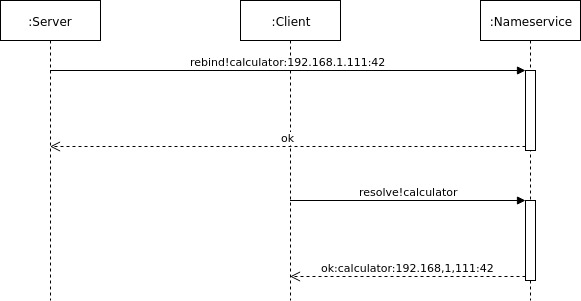
\includegraphics[scale=0.7]{../pictures/FlowChartNameService.jpg}\\
\centerline{\textbf{Abbildung 5:} Flowchart Nameservice}\\

\section{Middleware}
Aufgabe der Middleware ist es, den Zugriff auf entfernte Objekte so zu ermöglichen, dass die benutzenden Objekte nicht merken, dass es sich um ein entferntes Objekt handelt.\\
Im folgenden werde ich alle Module, die die Middleware beinhaltet, vorstellen.

\subsection{Object Broker}
Das "Frontend"  der Middleware.\\
Wird clientseitig von dem Stub-Objekt, das vom IDL-Compiler erzeugt wurde, angesprochen. Dieser clientseitige Object Broker sendet eine Anfrage mit dem Namen des Stub  Objektes an den Nameservice. Dieser liefert, sofern bekannt, die Hostadresse und den Port des Servers, auf dem das angefragte Objekt liegt, zurück.\\
Bekommt der anfragende ObjectBroker eine Hostadresse und einen Port zurück, stellt er dort eine Anfrage zur Ausführung der gewünschten Funktion. Der serverseitige Object Broker nimmt diese Anfrage entgegen und startet einen Dispatcher mit dem Socket des Clients.

\subsection{Dispatcher}
Der Dispatcher verarbeitet die Anfrage des Clients und ruft die angeforderte Methode des Objektes mit den übergebenen Parametern aus und leitet das Ergebnis oder auftretende Exceptions an den Client weiter. Danach wird die Verbindung geschlossen.

\subsubsection{Ablauf}
\begin{enumerate}
\item Empfangen der Nachricht vom Client
\item Auslesen des Namens vom Objektes, das angesprochen werden soll.
\item Anfrage an das Object Warehouse nach dem Objekt mit dem gegebenen Namen
\item Aufruf der angegebenen Methode
\item Rückgabe des Ergebnisses an den Client als Nachricht
\end{enumerate}

\subsection{Socket Controller}
Ist für die eigentliche Kommunikation verantwortlich. Sendet und empfängt Nachrichten über einen übergebenen Socket.

\subsubsection{Send Message}
\textbf{Beschreibung:}\\
Sendet eine Nachricht an das Objekt auf der "anderen Seite" des Sockets.\\ \\
\textbf{Aufruf:} sendMessage(String message)\\ \\
\textbf{Variablen}
\begin{enumerate}
\item \textbf{message:} Nachricht, die an den Kommunikationspartner gesendet werden soll
\end{enumerate}
\textbf{Ablauf}
\begin{enumerate}
\item Senden der übergebenen Nachricht an den Kommunikationspartner
\end{enumerate}

\subsubsection{Receive Message}
\textbf{Beschreibung:}\\
Empfängt eine Nachricht vom Kommunikationspartner.\\ \\
\textbf{Aufruf:} receiveMessage()\\ \\
\textbf{Ablauf}
\begin{enumerate}
\item Empfangen einer Nachricht an den Kommunikationspartner
\item Rückgabe der empfangenen Nachricht
\end{enumerate}

\subsection{Nameservice Interface}
Interface, dass den Nameservice anspricht.

\subsubsection{Rebind}
\textbf{Beschreibung:}\\
Spricht die Funktion Rebind des Nameservice an. Das Objekt wird mit Hilfe eines MWare-Objektes im Object Warehouse gespeichert und die IP-Adresse und der Port des Servers mit dem Namen des Objektes beim Nameservice registriert. \\ \\
\textbf{Aufruf:} rebind(Object servant, String name)\\ \\
\textbf{Variablen}
\begin{itemize}
\item \textbf{servant:} Objekt, dass beim Nameservice registriert wird
\item \textbf{name:} Name des Objektes, mit dem es beim Nameservice registriert wird
\end{itemize}
\textbf{Ablauf}
\begin{enumerate}
\item Erzeugen eines MWare-Objektes mit dem übergebenen Objekt
\item Einfügen des MWare-Objektes in das MWare Warehouse
\item Rebind-Anfrage an den Nameservice
\begin{itemize}
\item \textbf{Anfrage:} rebind!<Name>:<Hostadresse>:<Port>
\begin{itemize}
\item Name: Name des zu registrierenden Objektes 
\item Hostadresse: Eigene IP-Adresse, auf der der Server horcht
\item Port: Port, auf dem der Server horcht
\end{itemize}
\item \textbf{Antwort:} ok
\end{itemize}
\end{enumerate}

\subsubsection{Resolve}
\textbf{Beschreibung:}\\
Spricht die Funktion Resolve des Nameservice an. Die IP-Adresse und der Port des Servers, auf dem das Objekt mit dem übergebenen Namen liegt, wird zurückgegeben. \\ \\
\textbf{Aufruf:} resolve(String name)\\ \\
\textbf{Variablen}
\begin{itemize}
\item \textbf{name:} Name des Objektes, dass beim Nameservice abgefragt wird
\end{itemize}
\textbf{Rückgabe:} Objektreferenz des angefragten (entfernten) Objektes\\ \\
\textbf{Ablauf}
\begin{enumerate}
\item Erzeugen eines MWare-Objektes mit dem übergebenen Objekt
\item Einfügen des MWare-Objektes in das MWare Warehouse
\item Rebind-Anfrage an den Nameservice
\begin{itemize}
\item \textbf{Anfrage:} rebind!<Name>:<Hostadresse>:<Port>
\begin{itemize}
\item Name: Name des zu registrierenden Objektes 
\item Hostadresse: Eigene IP-Adresse, auf der der Server horcht
\item Port: Port, auf dem der Server horcht
\end{itemize}
\item \textbf{Antwort:} ok
\end{itemize}
\end{enumerate}

\subsection{Object Warehouse}
Verwaltet sowohl lokale aus auch entfernte Objekte für den Zugriff.

\subsubsection{Add Object}
\textbf{Beschreibung:}\\
Fügt ein Objekt zum Warehouse hinzu. \\ \\
\textbf{Aufruf:} addObject(String name, MWareObject object)\\ \\
\textbf{Variablen}
\begin{itemize}
\item \textbf{name:} Name des Objektes, dass hinzugefügt werden soll
\item \textbf{object:} Objektes, dass hinzugefügt werden soll
\end{itemize}
\textbf{Rückgabe:} Boolean, ob das Objekt hinzugefügt wurde, oder nicht.\\ \\
\textbf{Ablauf}
\begin{enumerate}
\item Prüfen, ob bereits ein Objekt mit dem Namen vorhanden ist
\begin{itemize}
\item Wenn ja: Rückgabe von false
\item Wenn nein: Hinzufügen des Objekts unter angegebenen Namen und Rückgabe von true
\end{itemize}
\end{enumerate}

\subsubsection{Remove Object}
\textbf{Beschreibung:}\\
Entfernt ein Objekt vom Warehouse. \\ \\
\textbf{Aufruf:} removeObject(String name)\\ \\
\textbf{Variablen}
\begin{itemize}
\item \textbf{name:} Name des Objektes, dass entfernt werden soll
\end{itemize}
\textbf{Rückgabe:} Boolean, ob das Objekt entfernt wurde, oder nicht.\\ \\
\textbf{Ablauf}
\begin{enumerate}
\item Prüfen, ob ein Objekt mit dem Namen vorhanden ist
\begin{itemize}
\item Wenn ja: Entfernen des Objektes und Rückgabe von true
\item Wenn nein: Rückgabe von false
\end{itemize}
\end{enumerate}

\subsubsection{Replace Object}
\textbf{Beschreibung:}\\
Fügt ein Objekt zum Warehouse hinzu. \\ \\
\textbf{Aufruf:} replaceObject(String name, MWareObject object)\\ \\
\textbf{Variablen}
\begin{itemize}
\item \textbf{name:} Name des Objektes, dass hinzugefügt werden soll
\item \textbf{object:} Objektes, dass hinzugefügt werden soll
\end{itemize}
\textbf{Ablauf}
\begin{enumerate}
\item Prüfen, ob bereits ein Objekt mit dem Namen vorhanden ist
\begin{itemize}
\item Wenn ja: Ersetzen des vorhandenen Objektes mit dem übergebenen
\item Wenn nein: Hinzufügen des Objekts unter angegebenen Namen
\end{itemize}
\end{enumerate}

\subsubsection{Get Object}
\textbf{Beschreibung:}\\
Liefert das Objekt mit dem übergebenen Namen zurück, sofern vorhanden. \\ \\
\textbf{Aufruf:} getObject(String name)\\ \\
\textbf{Variablen}
\begin{itemize}
\item \textbf{name:} Name des Objektes, dass hinzugefügt werden soll
\end{itemize}
\textbf{Rückgabe:} Objekt mit dem übergebenen Namen, wenn vorhanden.\\ \\
\textbf{Ablauf}
\begin{enumerate}
\item Prüfen, ob bereits ein Objekt mit dem Namen vorhanden ist
\begin{itemize}
\item Wenn ja: Rückgabe des Objekts
\item Wenn nein: Rückgabe von null
\end{itemize}
\end{enumerate}

\subsection{MWareObject}
Kann sowohl ein lokales, als auch ein entferntes Objekt repräsentieren und ruft die Methoden des Objektes auf.

\subsubsection{Call Method}
\textbf{Beschreibung:}\\
Ruft die in der übergebenen Nachricht angegebene Methode mit den angegebenen Parametern auf. \\ \\
\textbf{Aufruf:} callMethod(String message)\\ \\
\textbf{Variablen}
\begin{itemize}
\item \textbf{message:} String mit allen Informationen zur aufgerufenen Methode
\begin{itemize}
\item \textbf{Format:} <Name>!<Methode>![Parameter:Datentyp]*
\end{itemize}
\end{itemize}
\textbf{Rückgabe:} Ergebnis des Methodenaufrufs als String.\\ 
\textbf{Format:} result:<Ergebnis>.\\ \\
\textbf{Ablauf}
\begin{enumerate}
\item Parsen des übergebenen Strings mittels des oben angegebenen Formats
\item Aufruf der angegebenen Funktion mit den übergebenen Parametern
\item Rückgabe des Ergebnisses im Format: result:<Ergebnis>
\end{enumerate}

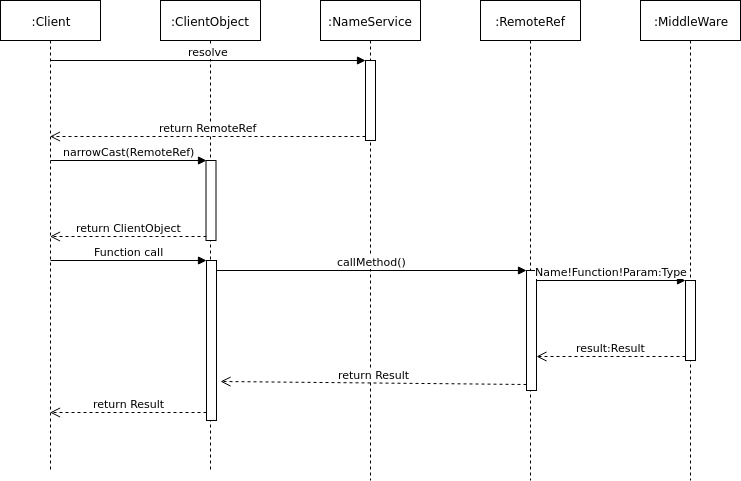
\includegraphics[scale=0.6]{../pictures/ClientFlowChart.jpg}\\
\centerline{\textbf{Abbildung 4:} Flowchart Client}\\

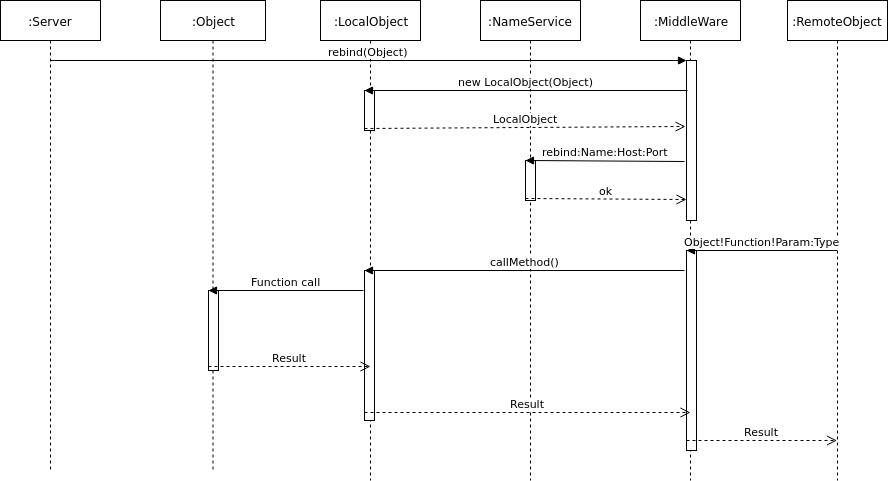
\includegraphics[scale=0.5]{../pictures/ServerFlowChart.jpg}\\
\centerline{\textbf{Abbildung 4:} Flowchart Server}

\section{IDL-Compiler}
Der IDL-Compiler muss die IDL-Datei einlesen und daraus zwei Java-Dateien erzeugen.
\begin{enumerate}
\item \_ClassNameImplBase.java - Abstrakte Klasse, die die Methoden der Klassen aus der IDL-Datei als abstrakte Methoden beinhaltet
\begin{enumerate}
\item Muss Methode narrowCast beinhalten, die ein Objekt zurückliefert, welches mittels des Objektes aus dem Resolve-Aufruf das RemoteObject ansprechen kann
\end{enumerate}
\item ClassName.java - Klasse, die die jeweiligen Methoden des entfernten Objektes aufruft.
\end{enumerate}
Die IDL-Datei ist folgendermaßen aufgebaut:
\begin{lstlisting}
module modulename {    // Name des Moduls
	class ClassA {    // Name der Klasse
		string methodA(int a);    // Methode der Klasse
	};    // Klassenende
	class ClassB {    // Zweite Klasse
		double methodA(double param1, double param2);
		int methodB(int param1);
	};
};    // Modulende
\end{lstlisting}

Das Modul beschreibt ein Java-Package, dass mehrere Klassen beinhalten kann. Dies muss mittels \\
package modulename;\\
in den Java-Klassen vermerkt werden.

\subsection{Abstrakte Klasse}

\subsubsection{narrowCast}
\textbf{Beschreibung:}\\
Liefert ein Objekt zurück, dass ein Objekt der erzeugten Klasse zurückliefert.\\ \\
\textbf{Aufruf:} sendMessage(Object rawObjectReference)\\ \\
\textbf{Variablen}
\begin{enumerate}
\item \textbf{rawObjectReference:} Objekt, dass vom Nameservice zurückgeliefert wird (MWareObject)
\end{enumerate}

\subsection{Ausführbare Klasse}
Die ausführbare Klasse muss alle Funktionen inklusive der Implementierung des Methodenaufrufs beinhalten. Siehe hierfür das Kapitel 2.3.6 CallMethod.